\documentclass[11pt]{article}
\usepackage[utf8]{inputenc}

\usepackage{amssymb,amsmath}
\usepackage{times,psfrag,epsf,epsfig,graphics,graphicx}
\usepackage{algorithm}
\usepackage{algorithmic}
\usepackage{xcolor}
\usepackage{tikz}

\newcommand\mybox[2][]{\tikz[overlay]\node[fill=blue!20,inner sep=2pt, anchor=text, rectangle, rounded corners=1mm,#1] {#2};\phantom{#2}}


\title{CSCI 338: Assignment~3~(7 points)}
\author{William Jardee}
\date{}


\begin{document}

\maketitle

\section*{Problem 1}

\noindent
Design context-free grammars for the following languages

(1.1) $A=\{a^nb^m|n\neq 2m\}$.

    \quad $S=aS_1bb | A | B$
    
    \quad $S_1 = aS_1 bb | A | B$
    
    \quad $A = aA|a$
    
    \quad $B=bB|b$
\newline


(1.2) $B=\{a^ib^jc^k|i,j,k\geq 0$ and either $i=j$ or $j=k\}$.

    \quad $S = S_1C|AS_2$
    
    \quad $S_1 = aS_1b | \varepsilon$
    
    \quad $S_2 = bS_2c | \varepsilon$
    
    \quad $A = Aa| \varepsilon$
        
    \quad $C = Cc| \varepsilon$
\newline


(1.3) $C=\{a^nb^m|n=3m\}$.

    \quad $S = aSbbb | \varepsilon$
\newline

(1.4) $D=\{a^nb^m|n\leq m+3\}$.

    \quad $S = AB|aAB|aaAB|aaaAB$
    
    \quad $A = aAb|\varepsilon$
    
    \quad $B= Bb | \varepsilon$
    
    
    
\newpage




\section*{Problem 2}

\noindent
Decide whether the following grammar is ambiguous.
\newline

$S\rightarrow AB|aaB$

$A\rightarrow a|Aa$

$B\rightarrow b$
\newline

\mybox[fill=blue!20]{This language is ambiguous}, as you can plot strings like ``$aab$" in two different routes. One option is to do
\[aaB \rightarrow b\]
or you could do 
\[AB \rightarrow Aa \rightarrow Aa \rightarrow b\]
Both give you ``$aab$" but in two different paths. 

\newpage

\section*{Problem 3}

\noindent
Convert the following CFG G to an equivalent PDA.

$R\rightarrow XRX|S$

$S\rightarrow aTb|bTa$

$T\rightarrow XTX|X|\epsilon$

$X\rightarrow a|b$
\newline

To actually make this solution readable I opted to not use the algorithm to expand links like ``$\varepsilon, R \rightarrow XRX$" into only one step pushes like ``$\varepsilon, R \rightarrow X$"; the algorithm would have been just a copy and paste step for me.The concept is still shown about how to build a $PDA$ from a $CFG$. \\

\begin{center}
    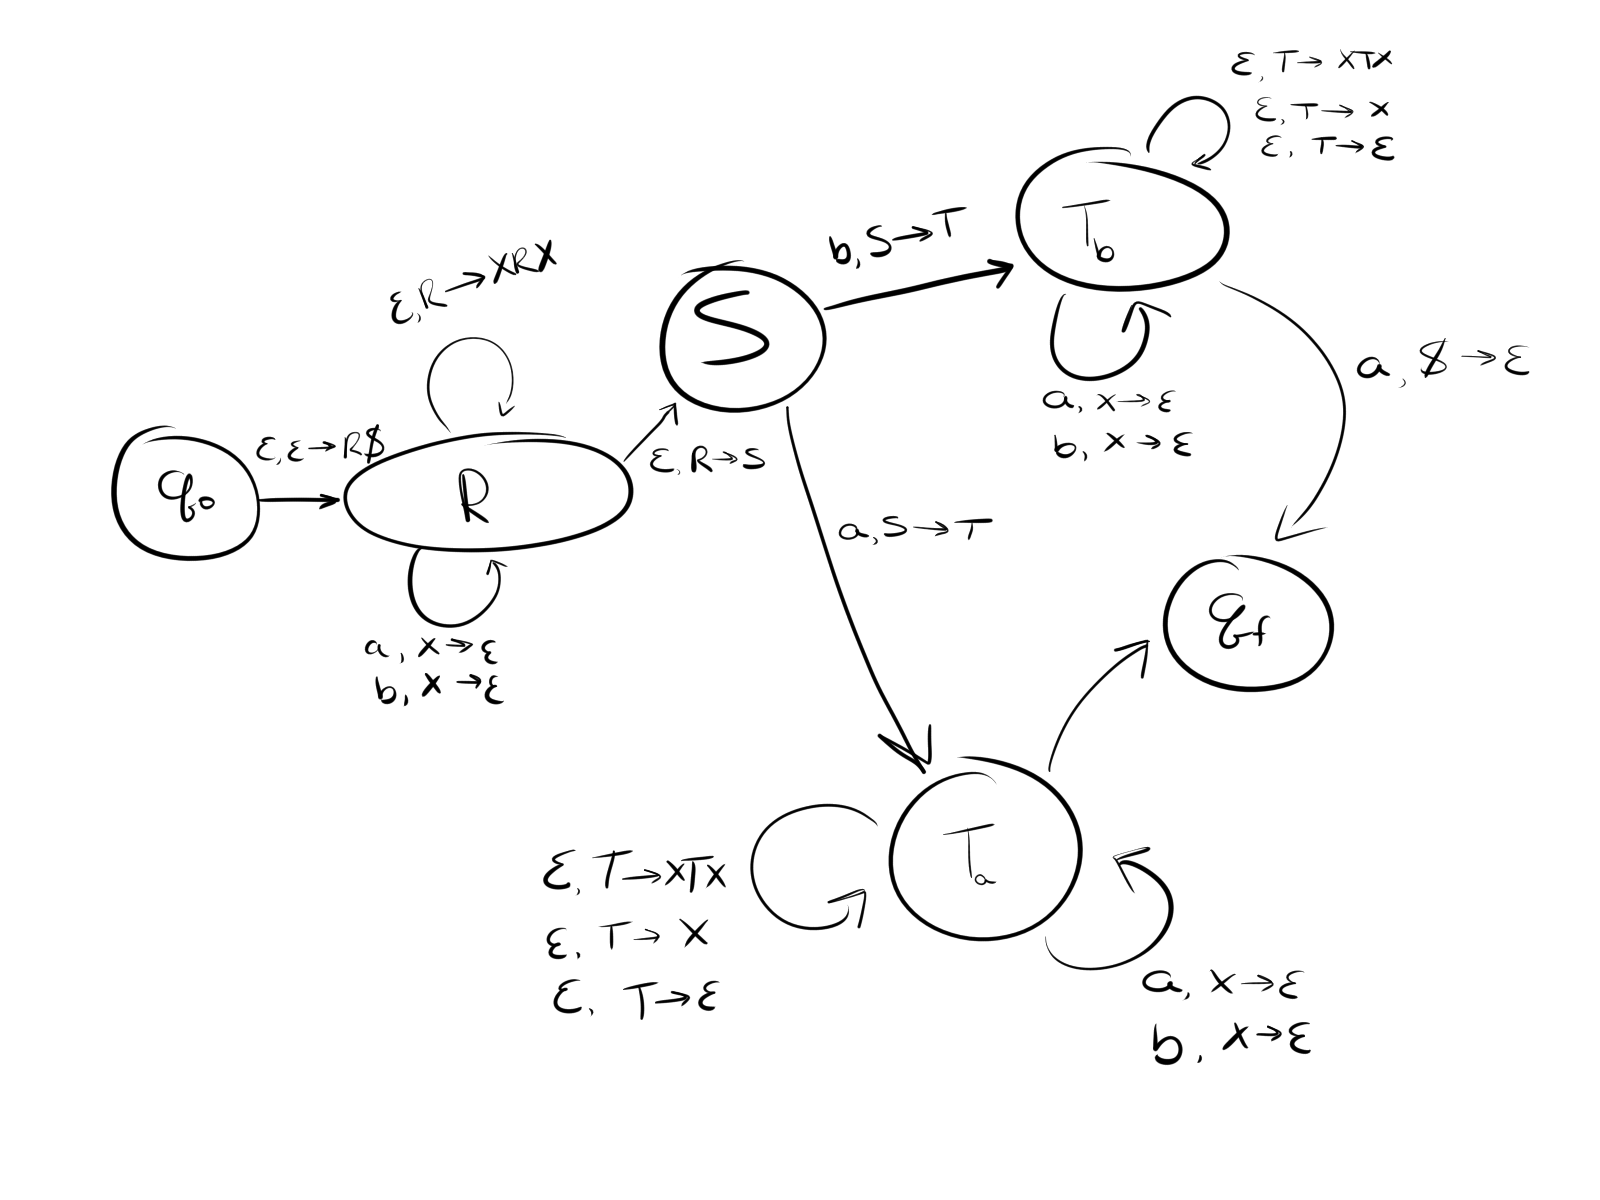
\includegraphics[width = 0.95\linewidth]{images/hw03_question03.png}
\end{center}



\newpage

\section*{Problem 4}

\noindent
Let $G=(V,\Sigma,R,S)$ be the following grammar. $V=\{S,T,U\}$;
$\Sigma=\{0,\#\}$; and $R$ is the set of rules:

$S\rightarrow TT|U$

$T\rightarrow 0T|T0|\#$

$U\rightarrow 0U00|\#$
\newline

\noindent
(4.1) Describe $L(G)$ in English.

If we take ``$\#$" as a defined part of our alphabet, then $L(G)$ describes
\[L(G) = \{((0^*\# \hphantom{l} 0^*)(0^*\# \hphantom{l} 0^*))\cup (0^j \# \hphantom{l} 0^{2j}) | j \geq 0\}\]

``Either two $\#$ with any number of $0$'s before the two or between them, or a $\#$ with double the number of $0$ after the symbol than before it."\\
\newline

\noindent
(4.2) Prove that $L(G)$ is not regular.\\

\textbf{Proof by Contradiction:}

Let us start by assuming, for the point of contradiction, that $G$ defines a regular language. Then we can apply the pumping lemma to $L(G)$, stating that there must be some $xy^i z$, s.t. $i\in \mathbb{Z}$, that is always valid in $L(G)$. We will focus on the second option started in part (4.1):  $\{(0^j \# \hphantom{l} 0^{2j}) | j \geq 0\}$; since the other condition is regular on its own. Let us take $s = 0^P\# \hphantom{l} 0^{2P}$. It is easy to see that $y^i$ must span either over the left set of $0^P$ or the right set of $0^{2P}$. If it didn't then there would be multiple copies of $\#$ when we do a pump up.

If $y^i$ is composed of $0$'s on either side of the $\#$, then we can do a pump down so that the right or left changes by a size greater than 0, let's say $X$. $2 \times P \pm X = 2P$ is only true when $X =0$, since $X \neq 0$, then our new string cannot be valid in $L(G)$. Thus, through contradiction, the grammar $G$ cannot describe a regular language. 
 
\begin{flushright}$\blacksquare$\end{flushright}



\newpage

\section*{Problem 5}

\noindent
Convert the following CFG into an equivalent CFG in Chomsky Normal Form

$A\rightarrow BAB|B|\varepsilon$

$B\rightarrow 00|\varepsilon$

    \quad $S_0 = AB_1|B_1A|B_1A_1|\varepsilon$
    
    \quad $A   = AB_1|B_1A|B_1A_1$
    
    \quad $A_1 = AB_1$
    
    \quad $B_1 = BB$
    
    \quad $B = 0$
\newline
    
\emph{Our definition  of the Chomsky Normal Form is built in such a way that it cannot accept an empty string, so I assumed we could deal with this in the first step as is in line with the Wiki page on Chomskey Normal Form.}

\newpage

\section*{Problem 6}

\noindent
Using pumping lemma to prove that the following languages are not
context-free.

(6.1) $L=\{a^nb^jc^k|k=nj\}$.
\newline

\textbf{Proof by Contradiction:}

Let us begin by assume that $L$ is a context-free language. Then, we can apply the pumping lemma for context-free languages to it. Let $s = a^P b^P c^{P^2}$. We have to be able to construct $s$ in such a way that $s = uv^i xy^i z$ where $|vy| > 0$, $|vxy| \leq P$, and the pumping condition of $i$. If $v$ or $y$ lie across a boundary of two different letters, then if we pump up then there will be a mixing of letters (i.e. if $v$ contains $a$'s and $b$'s such that $v=a^l b^m$, then if we do $v^2$ then we will have $a^l b^m a^l b^m$, which is not a valid sub-string of $L$. So, $v$ and $y$ must, individually, be composed of a single letter type. Since $|vxy| \leq P$, then we have three options: a) $v$ is composed of $b$'s and $y$ is composed of $c$'s, b) $v$ and $y$ are both composed of $b$'s, or c) $v$ and $y$ are both composed of $c$'s.

a) Here we can do a pump up. By pumping up we will be adding a certain number of $b$'s, $\alpha$, and another number of $c$'s, $\beta$; where $\alpha, \beta < P$. We must conserve the initial condition that $k=nj$, so let us check that. The right ($nj$) becomes $n(j+\alpha) = nj + \alpha n$ and the left becomes $k + \beta$. So, $\alpha n = \alpha P= \beta$. Since $\alpha \in \mathbb{Z}$, then $\beta \geq P$. This is a contradiction, so $s$ cannot be comprised of both $b$'s and $c$'s.

b) Let us say that $s = c^lcc^l$, where this $l$ is not the same $l$ we were referring to earlier. Let us pump down. Them the length of our new $k = P^2 - 2l = nj = P^2$. So our string only exists in $L$ if $l = 0$, which would violate one of the conditions of the pumping lemma, so this is a contradiction.

c) Let us finally say that $s = b^m b b^m$, where this m is not the same $m$ we were referring to earlier. Let us pump down. the length of our new $j= P - 2m$. Let us see about the $k = nj$ condition: $k = P^2 = P(P-2m) = P^2 - 2Pm$. The condition only holds if $m =0$, which is a contradiction to the pumping lemma. 

So, there is no possibility for $s$, such that our string stays in $L$ under the pumping lemma. Thus, by contradiction, $L$ is not context-free. 

\begin{flushright}$\blacksquare$\end{flushright}

\newpage

(6.2) $L=\{a^nb^j|n\geq (j-1)^3\}$.
\newline

\textbf{Proof by Contradiction:}


Let us begin by assuming that $L$ is a context-free language. Then, we can use the pumping lemma on it. Let $s = a^{P^3}b^P$. If we let $v$ of $y$ straddle $a$'s and $b$'s then we encounter the mixing issue that was dealt with in 6.1. So, $v$ and $y$ must independently be comprised of one type of letter. 

a) If we let $vxy$ exist only with $b$'s, then we pump up $v$ and $y$ a significantly large number, $r$, of times so that the number of $b$'s satisfy $P^3<((P+3i\times r)-1)^3$. Then we are no longer in $L$ and have reached a contradiction in this path.

b) If we let $vxy$ exist only with $a$'s, then we pump down such that the number of $a$'s, $n$, is zero. So, $0<(P-1)^3$, and we are no longer in $L$.

c) If we let $v$ be only $a$'s and $y$ only $b$'s, when we pump up we will be applying the same number of each letter to the string, keeping appropriate order. Let us say $|v| = \alpha$ and $|y| = \beta$. Then after an arbitrary number of pumps, $k$, the length of $n = P^3+ k\alpha$ and the length of $j = P +k \beta$. We see the comparison $n \geq (j-1)^3$ breaks down for significantly large $k$, since the $k\alpha$ term will grow linearly and the $k\beta$ term will grow cubically. So  this will eventually grow so that $s \notin L$. 

Thus we have show that there is no string $s$ that exists that can satisfy the pumping lemma, so we have reached a contradiction. So, $L$ is not a context-free language. 

\begin{flushright}$\blacksquare$\end{flushright}

\end{document}

